%% bare_conf.tex
%% V1.4
%% 2012/12/27
%% by Michael Shell
%% See:
%% http://www.michaelshell.org/
%% for current contact information.
%%
%% This is a skeleton file demonstrating the use of IEEEtran.cls
%% (requires IEEEtran.cls version 1.8 or later) with an IEEE conference paper.
%%
\documentclass{IEEEtran}
\usepackage[spanish]{babel}
\usepackage[utf8]{inputenc}
\usepackage{enumerate}
\usepackage{cite}
\usepackage{graphicx}  
\usepackage{subfig}

\graphicspath{ {./images/} }

% correct bad hyphenation here
\hyphenation{op-tical net-works semi-conduc-tor}


\usepackage{graphicx}
\begin{document}
%
% paper title
% can use linebreaks \\ within to get better formatting as desired
% Do not put math or special symbols in the title.
\title{Computación paralela y distribuida\\Práctica 1}


% author names and affiliations
% use a multiple column layout for up to three different
% affiliations
\author{\IEEEauthorblockN{Angel Rendón, Andrés Forero\\}
\IEEEauthorblockA{Universidad Nacional Bogotá, Colombia \\
Email:amrendonsa@unal.edu.co, afforeroc@unal.edu.co\\}
}

% make the title area
\maketitle

\begin{figure}[!t]
\centering

\includegraphics[width=\linewidth]{escudo.png}
\caption{Escudo de la Universidad.}
\label{fig_sim}
\end{figure}

% As a general rule, do not put math, special symbols or citations
% in the abstract
\begin{abstract}
Informe de práctica que muestra la influencia del uso de hilos de paralelización de cómputo y el tamaño de kernel de procesamiento de imágen sobre el tiempo de respuesta y el speedup en una implementación del efecto borroso en tres archivos *.bmp con resolución: 720p, 1080p y 4k. El código fuente implementa hilos POSIX, memoria dinámica y estructuras de datos para el cálculo de tiempo.
\end{abstract}

% no keywords

% For peer review papers, you can put extra information on the cover
% page as needed:
% \ifCLASSOPTIONpeerreview
% \begin{center} \bfseries EDICS Category: 3-BBND \end{center}
% \fi
%
% For peerreview papers, this IEEEtran command inserts a page break and
% creates the second title. It will be ignored for other modes.
\IEEEpeerreviewmaketitle

\section{Introducción}
% no \IEEEPARstart
Partiendo del concepto de computación paralela se dispuso a implementar un algoritmo de efecto borroso para imágenes de alta calidad y sobre este, estudiar el efecto combinado de hilos y kernel sobre el tiempo de respuesta. Lo anterior se hace de suma importancia debido a la eficiencia en el procesamiento de imágenes que tienen como condiciones: soportar los archivos de visual de gran tamaño soportado por el hardware que disponible actualmente en el modelo de computación clásica.
% You must have at least 2 lines in the paragraph with the drop letter
% (should never be an issue)
        

\hfill      
 
\hfill Mayo 7 de 2019

\section{Efecto borroso}
Cuando desenfocamos una imágen, hacemos que la transición entre colores de los pixeles que la componen sea más suave.

\begin{itemize}
\item Efecto borroso promedio: Toma un pixel referente y sobre un conjunto de pixeles alrededor promedia cada unos de los canales de colores de RGB para el pixel referente. El conjunto de pixeles alrededor puede varian en tamaño; esto se llama kernel. Y el promedio se realiza sobre todos los pixeles de la imágen.
\item Efecto borroso gaussiano: Es similar al efecto borroso promedio pero el promedio de los canales de colores se calcula con distintos pesos en función de la cercanía del pixel referencia.
\end{itemize}

\section{Paralelización del algoritmo}
La paralelización se logró primero construyendo el algoritmo de efecto borroso de forma secuencial y después aplicando el número de hilos dentro de su forma encapsulada. La forma encapsulada usa como argumentos de entradas los mismos que la función main y tiene como función nuclear void llamada parallel que es la que hace el promedio de los canales de colores para cada pixel.

\section{Experimentos y resultados}
El script itera entre los diferentes valores del kernel de procesamiento de imágen y el número de hilos para los 3 resoluciones. El programa toma estos valores como argumento paraleliza y finalmente arroja un valor de tiempo que es anexado a un documento *.csv. El archivo contiene todos los valores de tiempo.

\begin{figure}[htp]
\centering
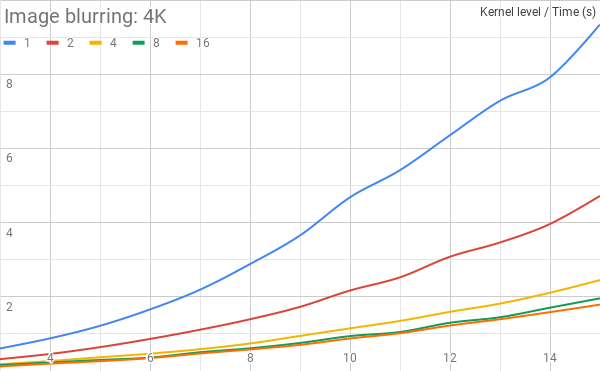
\includegraphics[width=\linewidth]{images/4k.png}
\caption{4K - Tiempo de respuesta: Kernel vs Hilos.}
\label{4kplot_time}
\end{figure}

\begin{figure}[htp]
\centering
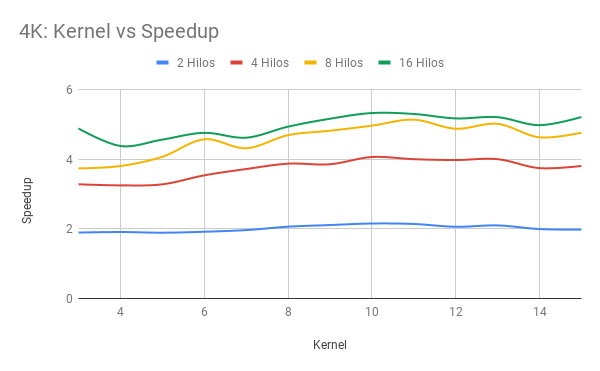
\includegraphics[width=\linewidth]{images/4K_Kernel_vs_Speedup.png}
\caption{4K - Speedup: Kernel vs Hilos}
\label{4kplot_speedup}
\end{figure}

\begin{figure}[htp]
\centering
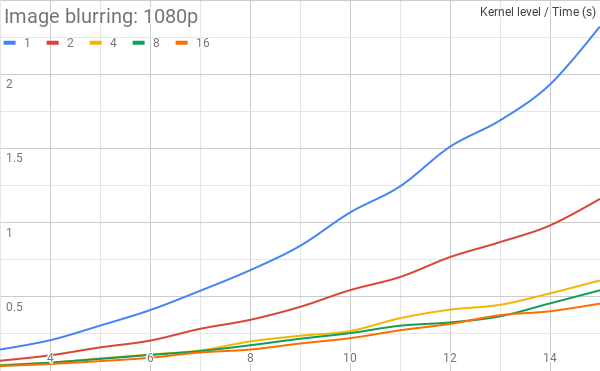
\includegraphics[width=\linewidth]{images/1080p.png}
\caption{1080p - Tiempo de respuesta: Kernel vs Hilos}
\label{1080pplot_time}
\end{figure}

\begin{figure}[htp]
\centering
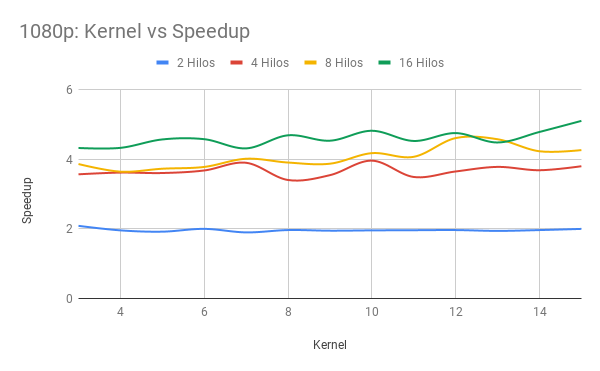
\includegraphics[width=\linewidth]{images/1080p_Kernel_vs_Speedup.png}
\caption{1080p - Speedup: Kernel vs Hilos}
\label{1080pplot_speedup}
\end{figure}

\begin{figure}[htp]
\centering
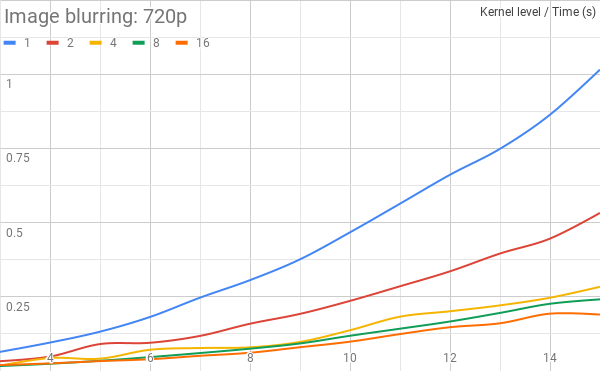
\includegraphics[width=\linewidth]{images/720p.png}
\caption{720p - Tiempo de respuesta: Kernel vs Hilos}
\label{720pplot_time}
\end{figure}

\begin{figure}[htp]
\centering
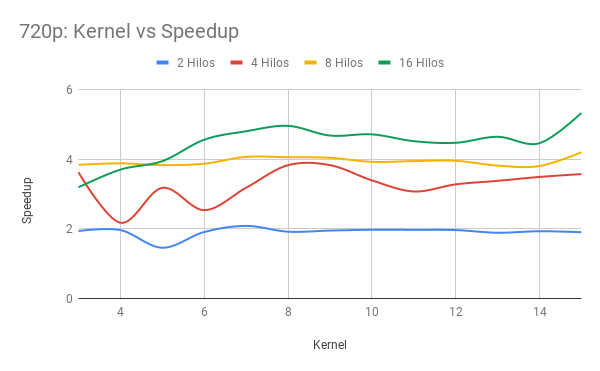
\includegraphics[width=\linewidth]{images/720p_Kernel_vs_Speedup.png}
\caption{720p - Speedup: Kernel vs Hilos}
\label{720pplot_speedup}
\end{figure}

\section{Conclusiones}
\begin{itemize}
\item El uso de varios hilos reduce la pendiente del tiempo de respuesta. El aumento de tiempo solo depende en mayor medida es del tamaño del kernel.
\item Hay una mejora en el tiempo de ejecución que depende solamente de la cantidad de hilos utilizado. Esto se nota más en imágenes de alta calidad.
\end{itemize}

\noindent 
\bibliographystyle{unsrt}       % APS-like style for physics

\bibliography{PARALELOS.bib}
\section{Bibliografía}
\begin{itemize}
\item https://www.w3.org/Talks/2012/0125-HTML-Tehran/Gaussian.xhtml
\item http://www.jhlabs.com/ip/blurring.html
\item https://computergraphics.stackexchange.com/questions/39/how-is-gaussian-blur-implemented
\end{itemize}

% that's all folks
\end{document}
